\chapter{March}

\section{Perceptron algorithm} \index{Perceptron algorithm}
Suppose we have input data $(x_1, y_1), (x_2, y_2), ..., (x_n, y_n) \in \mathbb{R}^p \times \{-1, 1\}$, 
and if the data points are separable, the perceptron algorithm works as following:

\begin{minted}[frame=lines, framesep=2mm,tabsize=4]{cpp}
w = 0
while some (x, y) is misclassified:
    w = w + yx
\end{minted}

\begin{remark}
In the separable case, perceptron algorithm guarantees to converge.
\end{remark}

\myheader{Multi-class perceptron}
\begin{minted}[frame=lines, framesep=2mm,tabsize=4]{cpp}
w_1 = w_2 = ... = w_k = 0
while some (x, y) is misclassified:
    for correct label y: w_y = w_y + x
    for incorrect label y*: w_(y*)  = w_(y*) - x
\end{minted}

\section{Kernel function} \index{Kernel function}
Following the perceptron algorithm, suppose $\phi$ is a function that maps $x$ to another feature space, such as $\phi(x) = (1, x_1, x_2, ..., x_1^2, x_2^2,..., x_1 x_2,...)$, which is a quadratic embedding.
In this case we can also run perceptron algorithm in the new feature space. 

\begin{minted}[frame=lines, framesep=2mm,tabsize=4]{cpp}
w = 0
while y*(w * \phi(x)) < 0:
w = w + y\phi(x)
\end{minted}

A problem is that every time we need to calculate $\phi(x)$, which may be of high dimensions. To solve this problem, we observe that in fact we don't need to access $\phi(x)$ at all to make a decision, instead we
can write $w$ as following:
\myequ{
    w = a_1 \phi(x_1) + a_2 \phi(x_2) + ... + a_n \phi(x_n)
}
then $w\cdot\phi(x)$ is a weighted sum of $\phi(x)\cdot\phi(x_i)$. In addition, we also observe that
\myequ{
    \phi(x) \cdot \phi(z) = (1 + x\cdot z)^2
}
That is, we don't need to calculate $\phi(x)$.


\myheader{kernel function} From above we know that we don't care about the embedding $\phi(x)$, we only 
care about the similarity between a pair of data points. Therefore, the kernel function is defined as following:
\vspace{0.5cm}
\begin{definition}[Kernel function]
    A function $k$: $\mathbb{R}^p \times \mathbb{R}^p \rightarrow \mathbb{R}$ is a valid kernel if it corresponds to some embedding, that is, there exists $\phi$ defined on $\mathbb{R}^p$ such that
    \myequ{
        k(x,z) = \phi(x) \cdot \phi(z)
        }
\end{definition}

This is equivalent to require that for any finite subset $\{x_1, x_2, ..., x_m\} \subset \mathbb{R}^p$,
the $m \times m$ similarity matrix 
\myequ{
    K_{ij} = k(x_i, x_j)
    }
is \textit{positive semidefinite}. Proof:
\myequ{
    Z^T K Z = Z^T (X^T X) Z = (XZ)^T (XZ) \geq 0
    }

\myheader{RBF kernel}
RBF kernel or Gaussian kernel is defined as
\myequ{
    k(x,z) = e^{-||x-z||^2 / 2\sigma^2}
    }

\myheader{string kernel}
For each substring $s$, we define feature:
\myequ{
    \phi_s(x) &= \# \text{ of times substring $s$ appears in $x$} \\
    \phi(x) &= (\phi_s(x): \text{ all strings } s)
    }


\section{$k$-means Clustering}\index{$k$-means Clustering}
\myheader{$k$-means} Minimize average squared distance between points and their nearest representatives.
The input is data points $x_1, x_2, ..., x_n$, and integer $k$, and the output is centers
$\mu_1, \mu_2, ..., \mu_k$.

\myheader{Lloyd's $k$-means algorithm}
\begin{minted}[frame=lines, framesep=2mm,tabsize=4]{cpp}
Initialize centers u_1, u_2, ... u_k in some manner.
Repeat until convergence:
    assign each point to its nearest center
    update each u_j to the mean of points assigned to it
\end{minted}

\myheader{How to initialize centers?} $k$-means++: start with extra centers, then prune later.

\begin{lstlisting}[
style=liststy,
]
Pick a data point x at random as the first center
Let $C = \{x\}$
	Repeat until the desired number of centers is attained:
	pick a data point $x$ at random from the following distributions: 
		$Pr(x) \propto dist(x, C)^2$, where $dist(x, C) = min_{z\in C}||x-z||$
	Add $x$ to $C$
\end{lstlisting}

\myheader{Streaming and online computation} If there are too much data to fit in memory, or the data
is continuously collected, we have to update the model gradually.

\myheader{The good and the bad} Good: fast and easy, effective in quantization. Bad: geared towards data in which the clusters are spherical, and of roughly the same results.

\section{Mixtures of Gaussians} \index{Mixtures of Gaussians}
Each of $k$ clusters is specified by a Guassian distribution $P_j = N(\mu_i, \sum_i)$ and a mixing weight
$\pi_j$. The overall distribution is a mixture of all Gaussians:
\myequ{
	Pr(x) = \pi_1 P_1(x) + \pi_2 P_2(x) + ... + \pi_k P_k(x)
}
We need to determine all the parameters including $\pi, \mu, \sum$. We apply \textbf{EM} algorithm to solve this problem
(see Figure~\ref{fig:em_mar}).
\begin{figure}[H]
	\centering{
		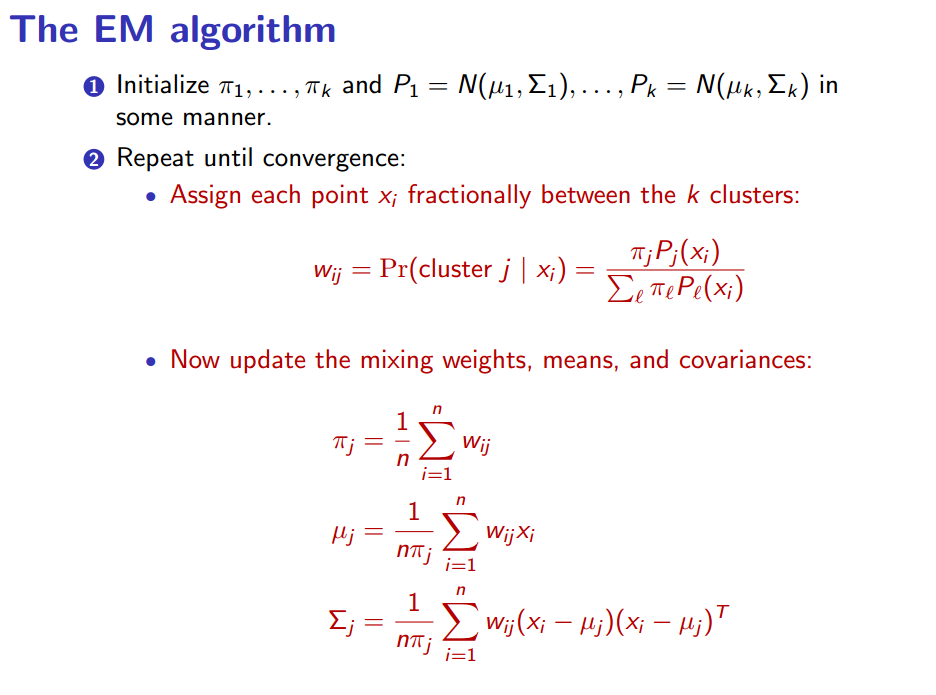
\includegraphics[width=0.9\textwidth]{./images/mar/gmm_em.PNG}
	}
	\caption{EM algorithm for GMM clustering.}
	\label{fig:em_mar}
\end{figure}

\section{Hierarchical clustering} \index{Hierarchical clustering}
Clustering is of multi-scale, and often there is no single right answer. Hierarchical 
clustering avoids these problems.
\begin{lstlisting}[
style=liststy,
]
Start with each point on its own
Repeat until there is just one cluster:
	Merge the two clusters with the $closest$ pair of points
Discard singleton clusters
\end{lstlisting}

\myheader{Linkage method} The problem is how we measure the distance
between two cluster of points.
\begin{enumerate}
	\item Single linkage: $dist(C, C') = min_{x \in C, x' \in C'} ||x - x'||$
	\item Complete linkage: $dist(C, C') = max_{x \in C, x' \in C'} ||x - x'||$
	\item Average linkage:
		\begin{enumerate}
			\item average pairwise distance between all pair of points in the two clusters
			\item distance between cluster centers
			\item Ward's method
		\end{enumerate}
\end{enumerate}


\section{Boosting}
\myheader{Adaboost} See Figure~\ref{fig:adaboost_mar}.
\begin{figure}[H]
	\centering{
		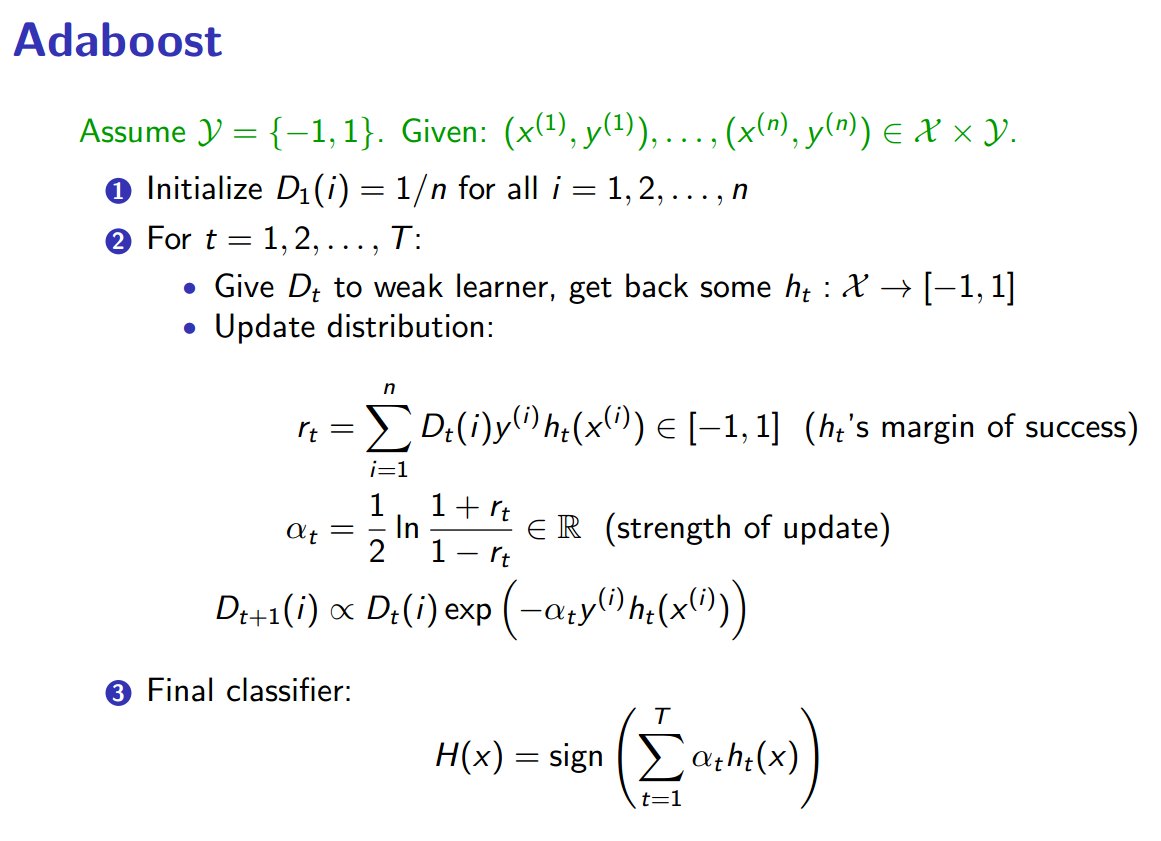
\includegraphics[width=0.9\textwidth]{./images/mar/adaboost.PNG}
	}
	\caption{Adaboost algorithms.}
	\label{fig:adaboost_mar}
\end{figure}

\myheader{Bagging} See Figure~\ref{fig:bagging_mar}
\begin{figure}[H]
	\centering{
		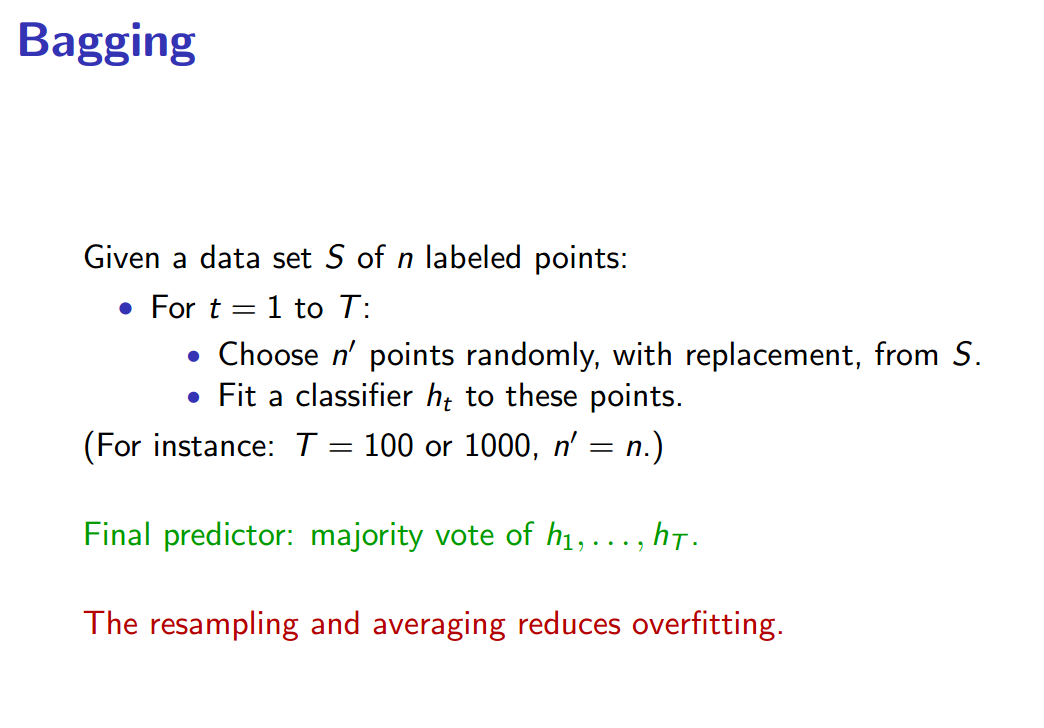
\includegraphics[width=0.9\textwidth]{./images/mar/bagging.PNG}
	}
	\caption{Bagging.}
	\label{fig:bagging_mar}
\end{figure}


\myheader{Random forest} See Figure~\ref{fig:random_forest_mar}
\begin{figure}[H]
	\centering{
		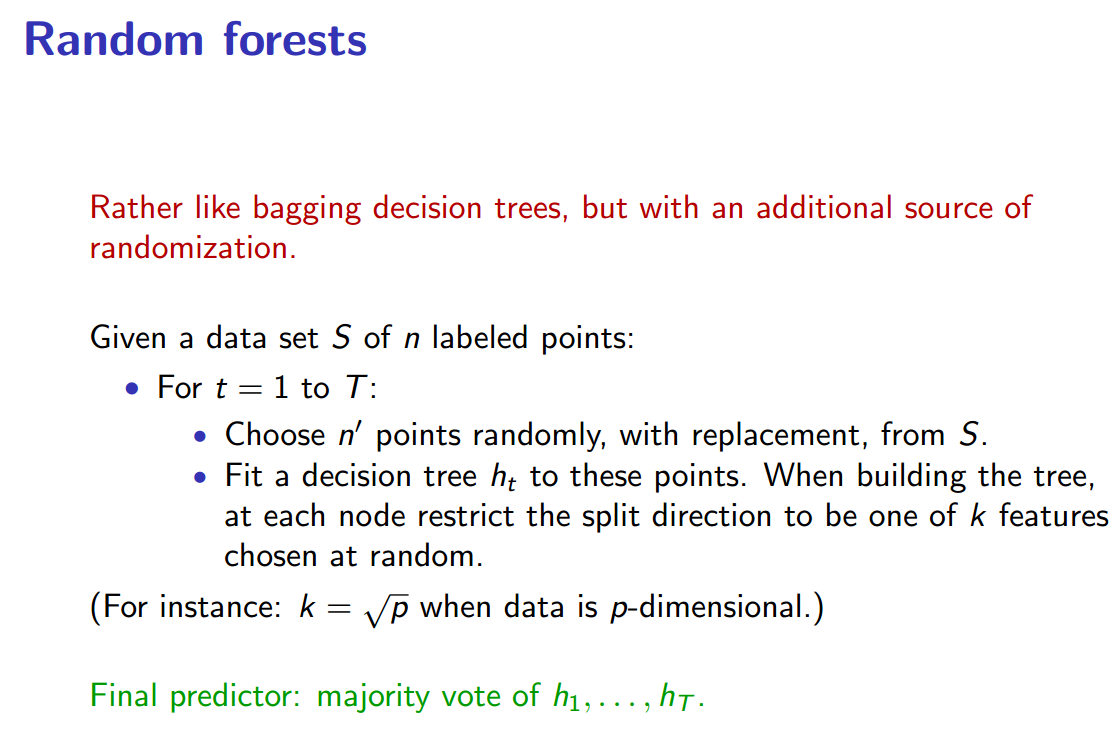
\includegraphics[width=0.9\textwidth]{./images/mar/random_forest.PNG}
	}
	\caption{Random forests.}
	\label{fig:random_forest_mar}
\end{figure}

\section{Informative projections} \index{Informative projections}

\myheader{Project to multiple directions} Suppose we want to project $x \in \mathbb{R}^p$
into the $k$-dimensional subspace spanned by $u_1, u_2, ..., u_k \in \mathbb{R}^p$, 
and suppose all $u_i$ are orthonormal (each has length one, and they are perpendicular to 
each other). Then the projection is:
\myequ{
	(x \cdot u_1)u_1 + (x \cdot u_2)u_2 + ... + (x \cdot u_k)u_k = UU^Tx
}

\myheader{Best single direction} Suppose we want to map our data $x_1, x_2, ..., x_n \in 
\mathbb{R}^p$ into just one dimension $x \mapsto u \cdot x$, what is the best direction $u$.

The best direction $u$ should be the one that maximize the variance after projection. Let $X$
be the data matrix, where each column is a data point, and $\sum$ be the covariance matrix of $X$. 
Suppose the mean of $X$ is $\mu \in \mathbb{R}^p$, then 
\myequ{
	\mathbb{E}(u^T X) & = u^T \mathbb{E}(X) = u^T \mu \\
	var(u^T X) & = \mathbb{E}(u^T X - u^T \mu) = \mathbb{E} (u^T (X - \mu) (X - \mu)^T u)  \\	
				& = u^T \mathbb{E}(X - \mu)(X - \mu)^T u = u^T \sum u
}

\begin{remark}
	$u^T\sum u$ is maximized by setting $u$ to the first \textbf{eigenvector} of $\sum$. The maximum
	value is the corresponding eigenvalue.
\end{remark}


\myheader{Best $k$-dimensional projection} Let $\sum$ be the $p\times p$ covariance matrix of $X$. 
and $\lambda_1 \geq  \lambda_2 \geq ... \geq \lambda_p$ are the eigenvalues, and $u_1, u_2, ...
u_p$ are the corresponding eigenvectors. Then the best $k$-dimensional projection directions are
$u_1, u_2, ..., u_k$.


\myheader{Spectral decomposition} See Figure~\ref{fig:spec_decomp_mar}.
\begin{figure}[H]
	\centering{
		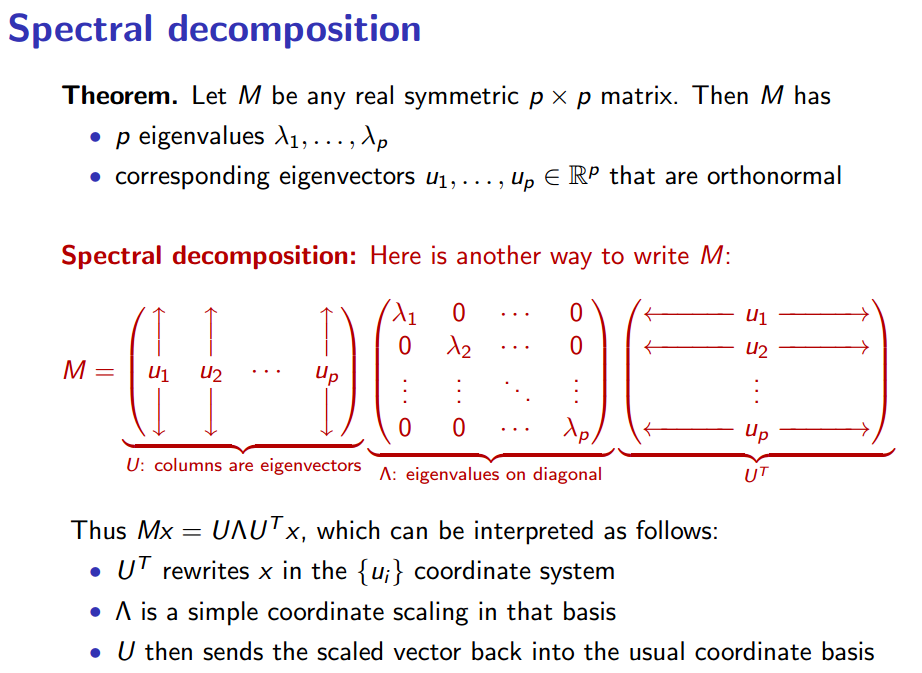
\includegraphics[width=0.9\textwidth]{./images/mar/spectral_decomp.PNG}
	}
	\caption{Spectral decomposition.}
	\label{fig:spec_decomp_mar}
\end{figure}

\myheader{Singular value decomposition (SVD)} See Figure~\ref{fig:svd_mar}. 
    Where $u_i, \sigma_i, v_i$ comes from? We know that:
    \begin{itemize}
        \item $Mv_i = \sigma_i u_i, M^T u_i = \sigma_i v_i$
        \item $M M^T u_i = \sigma_i^2 u_i, M^T M v_i = \sigma_i^2 v_i$
    \end{itemize}
    Therefore, $v_i$ is the eigenvectors of $M^T M$, and $u_i$ is the eigenvectors
    of $M M^T$. $MM^T$ and $M^TM$ has the same eigenvalues $\sigma_i^2$.  Note
    that all $\sigma_i$ are \textbf{non-negative}.

\begin{figure}[H]
	\centering{
		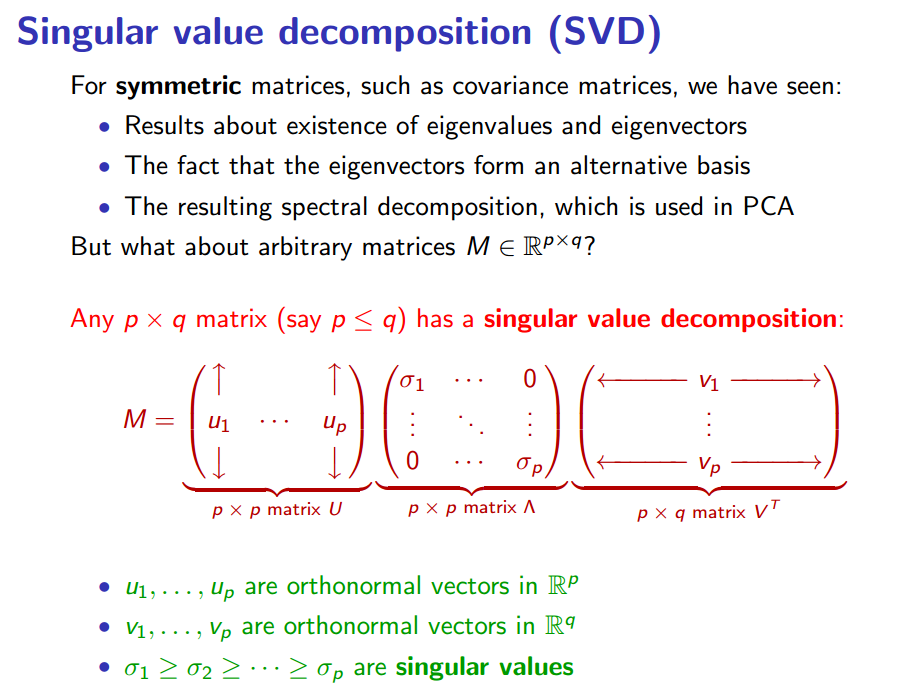
\includegraphics[width=0.9\textwidth]{./images/mar/SVD.PNG}
	}
	\caption{Singular value decomposition.}
	\label{fig:svd_mar}
\end{figure}

\section{Positive definite matrix }
\vspace{0.5cm}
\begin{definition}[Positive definite matrix]
    A square $p \times p$ symmetric matrix $A$ is positive definite if for all
    nonzero $x \in \mathbb{R}^p$,
    \myequ{
        x^T A x > 0
        }
\end{definition}

\myheader{Properties of positive definite matrix}
\begin{enumerate}
    \item The $r \times r$ submatrix $A_r$ (start from top left element) is also positive
    semidefinite.
    \item The $p$ eigenvalues of A $\lambda_1, \lambda_2, ..., \lambda_p$ are positive.
    Conversely, if all the eigenvalues of a matrix $B$ are
    positive, then $B$ is positive definite.
    
    \item There exist a unique decomposition of $A = LL^T$, where $L$ is a lower triangular
    matrix. This is called \textit{Cholesky Decomposition}. 
    \item There exists a unique decomposition of $A = VDV^T$.
    
\end{enumerate}
        
  

\section{Beyond projections} \index{Beyond projections}
Sometimes data in a high-dimensional space $\mathbb{R}^p$ in fact
lies close to a $k$-dimensional manifold, for $k\ll p$.

\myheader{ISOMAP algorithm}
Given data $x_1, x_2, ..., x_n$,
\begin{enumerate}
\item estimate \textit{geodesic distances} between the data points, that is, distance along the manifold.
\item embed these points in Euclidean space so as to match these distances.
\end{enumerate}

\myheader{Geodesic distances}
To estimate geodesic distances:
\begin{enumerate}
   \item Construct neighborhood graph, connect nodes whenever two nodes are close together.
   \item Compute distance in this graph (shortest-path algorithm).  
\end{enumerate}

\myheader{Distance-preserving embeddings} Problem definition:
\begin{lstlisting}[
style=liststy,] 
Input:an $n\times n$ matrix of pairwise distances $D$, where $D_ij$ is the distance between 
points $i$ and $j$.
Output: an embedding $z_1, z_2, ..., z_n \in \mathbb{R}^k$ that realizes these distances as closely as 
possible.
\end{lstlisting}

\myheader{Gram matrix}
Gram matrix on a set of vectors $z_1, z_2, ..., z_n$ is the matrix $B$ where
$B_{ij} = z_i \cdot z_j$.

\myheader{Classical multidimensional scaling} See Figure~\ref{fig:cms_mar}

\begin{figure}[H]
    \centering{
        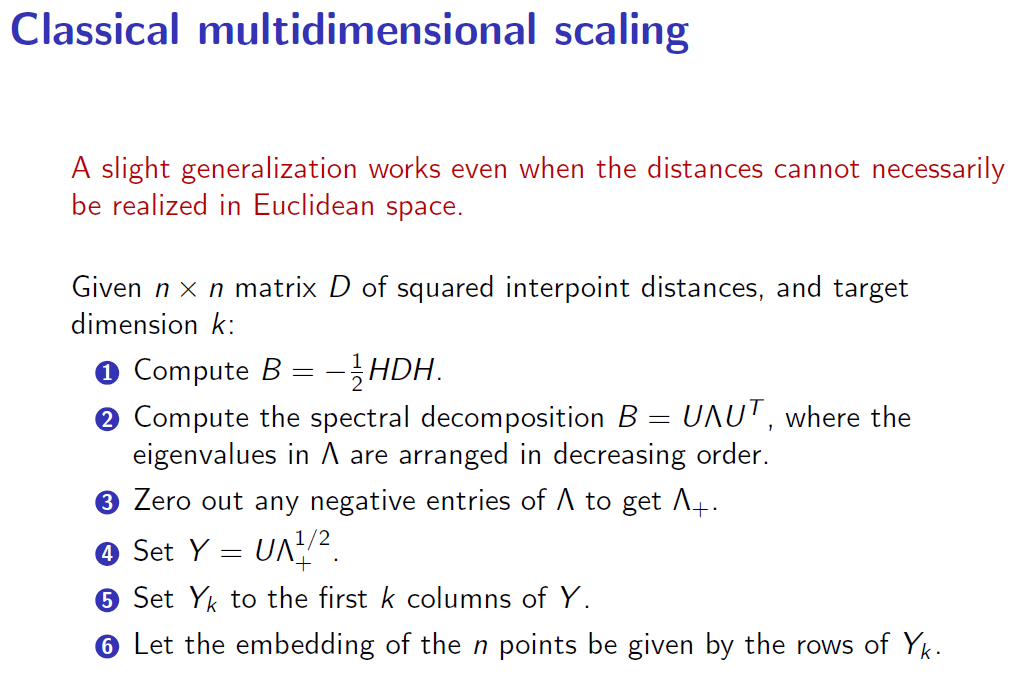
\includegraphics[width=0.9\textwidth]{./images/mar/cms.PNG}
    }
    \caption{Classical multidimensional scaling.}
    \label{fig:cms_mar}
\end{figure}


\section{Jacobian matrix} \index{Jacobian matrix}
In vector calculus, the Jacobian matrix is the matrix of all first-order partial derivatives of a vector-valued function.
\myequ{
    J  = \frac{d \mathbf{f}}{d \mathbf{x}} &= \begin{bmatrix}
        \frac{\partial \mathbf{f}}{\partial x_1} &
         \frac{\partial \mathbf{f}}{\partial x_2} &
         \dots & \frac{\partial \mathbf{f}}{\partial x_n} 
    \end{bmatrix}    \\
    & = \begin{bmatrix}
        \frac{\partial f_1}{\partial x_1} &
        \dots &
        \frac{\partial f_1}{\partial x_n} \\
         \vdots & \ddots & \vdots \\
         \frac{\partial f_m}{\partial x_1}  &
         \dots &
         \frac{\partial f_m}{\partial x_n} 
    \end{bmatrix}
}

\section{Gaussian-Newton algorithm} \index{Gaussian-Newton algorithm}
The Gaussian-Newton algorithm is used to solve non-linear least square problems. It is a modification
of Newton's method for finding a minimum of a function. Unlike Newton's method, the Gaussian-Newton algorithm
can only be used to minimize a sum of squared function values, but it has the advantage that the second
derivatives, which can be challenging to compute, are not required.

Given $m$ functions $r = (r_1, r_2, \dots, r_m)$ (often called residuals) of $n$ variables $\mathbf{\beta} = (\beta_1, \dots, \beta_n)$ with $m \geq n$, the Gauss–Newton algorithm iteratively finds the value of the variables which minimizes the sum of squares:
\myequ{
  S(\beta) = \sum\limits_{i=1}^{m} r_i^2(\beta)
} 
Start with an initial guess $\mathbf{\beta}^{(0)}$, the method proceeds by the iterations:
\myequ{
    \mathbf{\beta}^{(s+1)} = \mathbf{\beta}^{(s)}    - (J_r^T J_r)^{-1} J_r^T r(\mathbf{\beta}^{(s)})    
}
where 
\myequ{
    (J_r)_{ij} = \frac{\partial r_i(\beta^{(s)})}{\partial \beta_j}
}
If $m = n$, the iteration simplifies to 
\myequ{
    \mathbf{\beta}^{(s+1)} = \mathbf{\beta}^{(s)}    - (J_r)^{-1} r(\mathbf{\beta}^{(s)})
}


\section{Functional programming: introductions} \index{Functional programming: introductions}

\myheader{Why FP?}
We want software to be \textit{readable, reusable, modifiable, predictable and checkable}. Functional
programming could satisfy these requirements. 

There is no assignment, mutation, or loop in FP.

\section{$\lambda$-calculus}\index{$\lambda$-calculus}
Lambda calculus (also written as $\lambda$-calculus) is a formal system in mathematical logic for expressing computation
 based on function abstraction and application using variable binding and substitution.

\myheader{Syntax}
Three kinds of expressions:
\begin{lstlisting}[
style=liststy,] 
e ::= x             
    | $\lambda$ x. e      
    | $\lambda$ e_1 e_2   
\end{lstlisting}
called \textit{variables}, \textit{functions}($\lambda$-abstraction), and \textit{application}.
Functions $\lambda x. e$ takes $x$ as an input and output $e$.
 
Application associates to the left: $x y z$ means $(x y) z$. However, abstraction extends as far right
as possible:
$\lambda x. x \lambda y. x y z \Rightarrow \lambda x. (x \lambda y. ((x y) z))$ 

Identity function: $I = \lambda x. x$

\myheader{Scope of identifier (variable)}
Scope of a variable is the part of program where the variable is \textit{accessible}.

$\lambda x. E$ binds variable $x$ in $E$:
\begin{enumerate}
    \item $x$ is the newly introduced varialbe.
    \item $E$ is the scope of $x$.
    \item $x$ is bound in $\lambda x. E$
\end{enumerate}

$y$ is \textit{free} if it occurs not bound in $E$:
\begin{enumerate}
    \item $Free(x) = \{x\}$
    \item $Free(E_1 E_2) = Free(E_1) \cup Free(E_2)$ 
    \item $Free(\lambda x. E) = Free(E) - \{x\}$
\end{enumerate}

$\alpha$-renaming:
\begin{enumerate}
    \item Allows bound variable names to be changed.
    \item $\lambda x. x = \lambda y. y$
\end{enumerate}

substitution:
\begin{enumerate}
    \item $[E'/x]E$: use $E'$ to substitute all $x$ bounded in $E$
    \item $[y (\lambda x. x)/x] \lambda y. (\lambda x. x) y x
           \equiv$
           $[y (\lambda v. v)/x] \lambda y. (\lambda u. u) z x $ (renaming)
           $\equiv \lambda z. (\lambda u. u) z (y (\lambda v. v))$ (substitution) 
\end{enumerate}























